\documentclass[aspectratio=43,11pt]{beamer}

\usepackage[utf8]{inputenc}
\usepackage[T1]{fontenc}

\usepackage{babel}
\babelprovide[import,main]{spanish}

\usepackage{amsmath,amssymb,bm}
\usepackage{tikz}
\usepackage{pgfplots}\pgfplotsset{compat=1.16}
\usepackage{booktabs}
\usepackage{colortbl}

\usetikzlibrary{arrows.meta,positioning,calc}

  \definecolor{oro}{HTML}{C8860B}
\definecolor{orosuave}{HTML}{E9C46A}
\definecolor{pizarra}{HTML}{22303C}
\definecolor{pizarra2}{HTML}{34495E}
\definecolor{gristexto}{HTML}{37474F}
\definecolor{grisclaro}{HTML}{ECEFF1}
\definecolor{rojohot}{HTML}{C0392B}

\usetheme{default}
\usefonttheme{structurebold}
\setbeamertemplate{navigation symbols}{}

\setbeamercolor{normal text}{fg=gristexto}
\setbeamercolor{structure}{fg=oro}
\setbeamercolor{frametitle}{fg=white,bg=pizarra}
\setbeamercolor{title}{fg=white}
\setbeamercolor{itemize item}{fg=oro}
\setbeamercolor{itemize subitem}{fg=oro}
\setbeamercolor{block title}{fg=white,bg=pizarra2}
\setbeamercolor{block body}{fg=gristexto,bg=grisclaro}
\setbeamercolor{alerted text}{fg=oro}

\setbeamertemplate{itemize item}{\small\raise0.3pt\hbox{\textbullet}}
\setbeamertemplate{itemize subitem}{\scriptsize\raise0.3pt\hbox{--}}
\setbeamertemplate{blocks}[rounded][shadow=false]

\setbeamertemplate{frametitle}{%
\nointerlineskip
  \begin{beamercolorbox}[wd=\paperwidth,ht=1.5em,dp=0.8em,leftskip=10pt]{frametitle}%
    \insertframetitle%
  \end{beamercolorbox}}
  % Número de diapositiva, abajo a la derecha
\setbeamertemplate{footline}{%
  \begin{beamercolorbox}[wd=\paperwidth,ht=2.5ex,dp=1.4ex,rightskip=12pt]{}%
    \hfill{\color{oro}\scriptsize\insertframenumber}%
  \end{beamercolorbox}%
}

\newcommand{\fondopizarra}{%
  \begin{tikzpicture}[remember picture,overlay]
    \fill[pizarra] (current page.south west) rectangle (current page.north east);
    \fill[oro] (current page.south west) rectangle ([yshift=4pt]current page.south east);
  \end{tikzpicture}}

\newcommand{\seccion}[1]{%
  {\setbeamertemplate{footline}{}%
  \begin{frame}[plain]\fondopizarra
    \vfill\centering{\color{white}\bfseries\Large #1\par}\vfill
  \end{frame}}}

\title{Simulaciones de la dispersión de luz por nanopartículas esféricas de oro}
\subtitle{Del formalismo de Mie a las nanoantenas ópticas}
\author{Gorka Larrazabal Epalza}
\date{Leioa, \today}

\begin{document}

% ============================ PORTADA ============================
{\setbeamertemplate{footline}{}
\begin{frame}[plain]
  \fondopizarra
  \vfill
  \begin{center}
    {\color{white}\bfseries\Large Simulaciones de la dispersión de luz por nanopartículas esféricas de oro\par}
    \vspace{6pt}
    {\color{orosuave}\itshape\large Del formalismo de Mie a las nanoantenas ópticas\par}
    \vspace{20pt}
    {\color{white}\large Gorka Larrazabal Epalza\par}
    \vspace{4pt}
    {\color{grisclaro}\footnotesize Trabajo Fin de Grado --- Grado en Física\par}
    \vspace{16pt}
    {\color{orosuave}\footnotesize Leioa, \today\par}
  \end{center}
  \vfill
  \begin{tikzpicture}[remember picture,overlay]
    \node[anchor=south east]
      at ([xshift=-1.1em,yshift=1.0em]current page.south east)
      {\includegraphics[height=1.5cm]{figs/EHU/altua/EHU_logotipo_negatiboa_ALTUA_tr.png}};
  \end{tikzpicture}
\end{frame}
}

% ============================ D1: MOTIVACIÓN ============================
\begin{frame}{Motivación}
  \vspace{10pt}
  \begin{itemize}
    \setlength{\itemsep}{16pt}
    \item Dispersión por esferas
    \item Nanofotónica
    \item \textit{Hot spots}
    \item Nanoantenas
  \end{itemize}
\end{frame}

% ============================ D2: OBJETIVOS ============================
\begin{frame}{Objetivos}
  \vspace{10pt}
  \begin{itemize}
    \setlength{\itemsep}{16pt}
    \item Teoría: Mie y T-matrix
    \item Análisis del código en Fortran (MSTM)
    \item Entorno propio en Python
    \item Aplicación: esfera, dímero, tetrámero $\to$ nanoantenas
  \end{itemize}
\end{frame}

% ============================ ÍNDICE ============================
\begin{frame}{Índice}
  \vspace{10pt}
  \begin{enumerate}
    \setlength{\topsep}{0pt}
    \setlength{\itemsep}{14pt}
    \item Desarrollo de la teoría necesaria: Mie y dispersión múltiple
    \item Exploración del código en Fortran
    \item Análisis del código en Python
    \item Exposición de resultados y enlace con las nanoantenas
    \item Conclusiones
  \end{enumerate}
\end{frame}

% =========================== D3: TEORÍA DE MIE ESQUEMA =========================
\begin{frame}{Teoría de Mie}
\centering
\vspace{14pt}
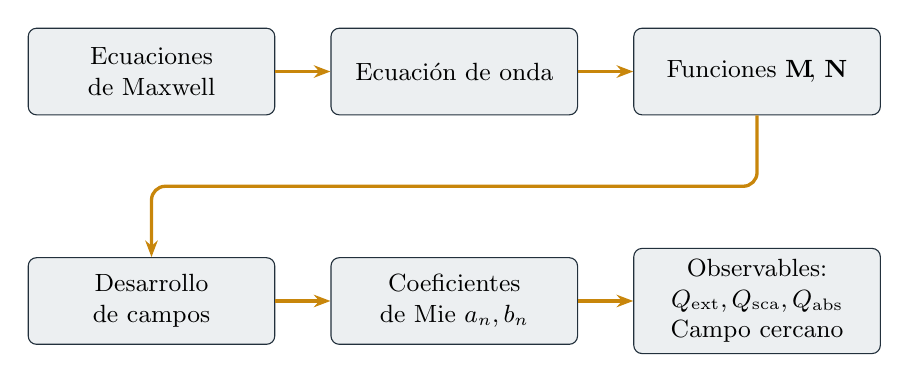
\begin{tikzpicture}[
  box/.style={
    draw=pizarra, fill=grisclaro, rounded corners=3pt,
    text width=2.85cm, align=center, minimum height=1.1cm,
    font=\small, inner sep=4pt
  },
  arr/.style={-{Stealth[length=6pt]}, thick, color=oro, line width=1.2pt}
]
  \node[box] (max) {Ecuaciones de Maxwell};
  \node[box, right=7mm of max] (ond) {Ecuación de onda};
  \node[box, right=7mm of ond] (nm)  {Funciones $\mathbf{M}$\!, $\mathbf{N}$};
  \draw[arr] (max) -- (ond);
  \draw[arr] (ond) -- (nm);
  \node[box, below=18mm of max] (des) {Desarrollo de campos};
  \node[box, right=7mm of des]  (mie) {Coeficientes de Mie $a_n,b_n$};
  \node[box, right=7mm of mie]  (obs) {Observables: $Q_\text{ext},Q_\text{sca},Q_\text{abs}$\\ Campo cercano};
  \draw[arr] (des) -- (mie);
  \draw[arr] (mie) -- (obs);
  \draw[arr, rounded corners=5pt]
    (nm.south) -- ++(0,-9mm) -- ($(des.north)+(0,9mm)$) -- (des.north);
\end{tikzpicture}
\begin{tikzpicture}[remember picture,overlay]
  \node[anchor=south west, text=pizarra2, font=\scriptsize]
    at ([xshift=10pt,yshift=8pt]current page.south west)
    {Bohren \& Huffman, \textit{Absorption and Scattering of Light by Small Particles}, Wiley (1983).};
\end{tikzpicture}
\end{frame}
% =========================== M y N + DESARROLLO + OBSERVABLES ============================
% --- Funciones M y N + desarrollo general ---
\begin{frame}{La base natural: funciones $\mathbf{M}$ y $\mathbf{N}$}
  \vspace{6pt}
  En simetría esférica, las soluciones de la ecuación de onda vectorial son dos
  familias de \alert{armónicos esféricos vectoriales}, $\mathbf{M}$ y $\mathbf{N}$.
  \vspace{4pt}

  Forman una \alert{base completa}: cualquier campo se desarrolla en ella.
  \vspace{4pt}
  \begin{equation*}
    \begin{aligned}
      \mathbf{E}_i = \sum_{m=0}^{\infty}\sum_{n=m}^{\infty}\big(
        & B_{emn}\mathbf{M}_{emn} + B_{omn}\mathbf{M}_{omn}+ A_{emn}\mathbf{N}_{emn} + A_{omn}\mathbf{N}_{omn}\big)
    \end{aligned}
  \end{equation*}
  \vspace{2pt}
  \begin{center}
    {\footnotesize\color{pizarra2} El problema se reduce a hallar los coeficientes del desarrollo.}
  \end{center}
\end{frame}

% --- Desarrollo de los campos en VSWF (reubicada desde el apéndice) ---
\begin{frame}{Desarrollo de los campos en VSWF}
  \vspace{2pt}
  \footnotesize
  \textbf{Campo incidente}:
  \begin{equation*}
    \mathbf{E}^{(i)} = E_0\sum_{n=1}^{\infty}i^n\frac{2n+1}{n(n+1)}
    \!\left(\mathbf{M}^{(1)}_{o1n} - i\,\mathbf{N}^{(1)}_{e1n}\right)
  \end{equation*}

  \textbf{Campo interno}:
  \begin{equation*}
    \mathbf{E}^{(int)} = \sum_{n=1}^{\infty}E_n
    \!\left(c_n\,\mathbf{M}^{(1)}_{o1n} - i\,d_n\,\mathbf{N}^{(1)}_{e1n}\right)
  \end{equation*}

  \textbf{Campo dispersado}:
  \begin{equation*}
    \mathbf{E}^{(sca)} = \sum_{n=1}^{\infty}E_n
    \!\left(i\,a_n\,\mathbf{N}^{(3)}_{e1n} - b_n\,\mathbf{M}^{(3)}_{o1n}\right)
  \end{equation*}

  \vspace{2pt}
  con $E_n = i^n E_0(2n+1)/[n(n+1)]$. Los coeficientes $a_n,\,b_n$ (Mie) se obtienen
  imponiendo continuidad de las componentes tangenciales en $r=a$.
\end{frame}

% --- Observables a partir de a_n, b_n ---
\begin{frame}{Observables: cálculo de eficiencias}
  \vspace{6pt}
  Conocidos $a_n$ y $b_n$ (con $x=ka$), se obtienen las \alert{eficiencias} de
  extinción, dispersión y absorción:
  \vspace{2pt}
  \begin{equation*}
    Q_\text{ext} = \frac{2}{x^2}\sum_{n=1}^{\infty}(2n+1)\,\mathrm{Re}(a_n+b_n)
  \end{equation*}
  \begin{equation*}
    Q_\text{sca} = \frac{2}{x^2}\sum_{n=1}^{\infty}(2n+1)\left(|a_n|^2+|b_n|^2\right)
  \end{equation*}
  \begin{equation*}
    Q_\text{abs} = Q_\text{ext} - Q_\text{sca}
  \end{equation*}
\end{frame}

% =================== D: MÚLTIPLES ESFERAS ESQUEMA =======================
\begin{frame}{Dispersión múltiple}
\centering
\vspace{14pt}
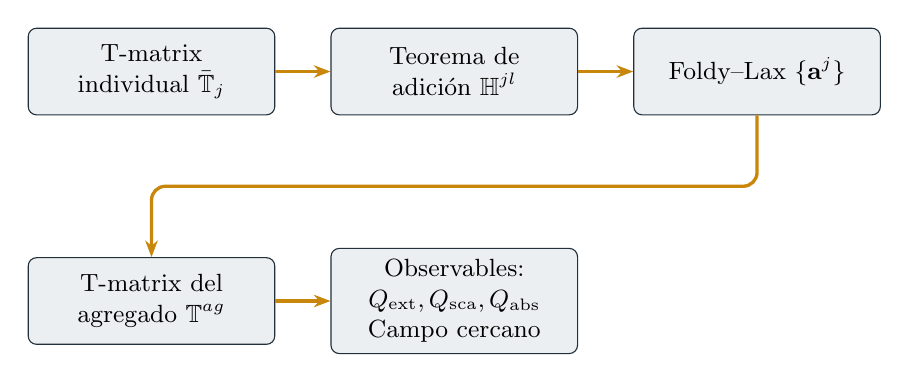
\begin{tikzpicture}[
  box/.style={
    draw=pizarra, fill=grisclaro, rounded corners=3pt,
    text width=2.85cm, align=center, minimum height=1.1cm,
    font=\small, inner sep=4pt
  },
  arr/.style={-{Stealth[length=6pt]}, thick, color=oro, line width=1.2pt}
]
  \node[box] (tm)  {T-matrix\\ individual $\bar{\mathbb{T}}_j$};
  \node[box, right=7mm of tm]  (add) {Teorema de adición $\mathbb{H}^{jl}$};
  \node[box, right=7mm of add] (fl)  {Foldy--Lax $\{\mathbf{a}^j\}$};
  \draw[arr] (tm)  -- (add);
  \draw[arr] (add) -- (fl);
  \node[box, below=18mm of tm] (tag) {T-matrix del agregado $\mathbb{T}^{ag}$};
  \node[box, right=7mm of tag] (obs) {Observables: $Q_\text{ext},Q_\text{sca},Q_\text{abs}$\\ Campo cercano};
  \draw[arr] (tag) -- (obs);
  \draw[arr, rounded corners=5pt]
    (fl.south) -- ++(0,-9mm) -- ($(tag.north)+(0,9mm)$) -- (tag.north);
\end{tikzpicture}
\end{frame}

% =========================== DISPERSIÓN MÚLTIPLE: PLANTEAMIENTO + FOLDY-LAX ============================

% --- T-matrix individual + campo excitante ---
\begin{frame}{Planteamiento: T-matrix y campo excitante}
  \vspace{6pt}
  \footnotesize
  La respuesta \alert{individual} de cada esfera relaciona su campo excitante
  $\mathbf{q}^{j}$ con el dispersado $\mathbf{a}^{j}$ a través de su T-matrix
  (diagonal, coeficientes de Mie):
  \begin{equation*}
    \mathbf{a}^{j} = \bar{\mathbb{T}}_j\,\mathbf{q}^{j},
    \qquad
    \bar{\mathbb{T}}_j = \mathrm{diag}\bigl(\ldots,\bar{a}_n^{j},\bar{b}_n^{j},\ldots\bigr)
  \end{equation*}
  \vspace{2pt}

  El \alert{teorema de adición} traslada las ondas salientes de la esfera $l$ al
  sistema de la esfera $j$ mediante el operador $\mathbb{H}^{jl}$:
  \begin{equation*}
    \mathbb{H}^{jl}
    =
    \begin{pmatrix}
      A^{jl} & B^{jl} \\
      B^{jl} & A^{jl}
    \end{pmatrix}
  \end{equation*}
  \vspace{2pt}

  Así, el campo que \alert{excita} a la esfera $j$ es el incidente más lo dispersado
  por todas las demás:
  \begin{equation*}
    \mathbf{q}^{j}
    = \mathbf{p}^{j}
    + \sum_{\substack{l=1\\l\neq j}}^{N_S}\mathbb{H}^{jl}\,\mathbf{a}^{l}
  \end{equation*}
\end{frame}

% --- Sistema acoplado de Foldy-Lax ---
\begin{frame}{El sistema acoplado de Foldy--Lax}
  \vspace{4pt}
  \footnotesize
  Sustituyendo $\mathbf{q}^{j}$ en $\mathbf{a}^{j}=\bar{\mathbb{T}}_j\mathbf{q}^{j}$
  se obtiene, para cada esfera:
  \begin{equation*}
    \mathbf{a}^{j}
    - \bar{\mathbb{T}}_j \sum_{\substack{l=1\\l\neq j}}^{N_S}
      \mathbb{H}^{jl}\,\mathbf{a}^{l}
    = \bar{\mathbb{T}}_j\,\mathbf{p}^{j},
    \qquad j = 1,\ldots,N_S
  \end{equation*}
  \vspace{2pt}

  que en forma matricial global es:
  \begin{equation*}
    \underbrace{
    \begin{pmatrix}
      \mathbb{I}                          & -\bar{\mathbb{T}}_1\mathbb{H}^{12} & \cdots & -\bar{\mathbb{T}}_1\mathbb{H}^{1N_S} \\
      -\bar{\mathbb{T}}_2\mathbb{H}^{21}  & \mathbb{I}                         & \cdots & -\bar{\mathbb{T}}_2\mathbb{H}^{2N_S} \\
      \vdots                              &                                    & \ddots & \vdots                               \\
      -\bar{\mathbb{T}}_{N_S}\mathbb{H}^{N_S 1} & \cdots                       &        & \mathbb{I}
    \end{pmatrix}}_{\mathbb{M}_{sys}}
    \begin{pmatrix}\mathbf{a}^1\\\mathbf{a}^2\\\vdots\\\mathbf{a}^{N_S}\end{pmatrix}
    =
    \begin{pmatrix}
      \bar{\mathbb{T}}_1\mathbf{p}^1\\
      \bar{\mathbb{T}}_2\mathbf{p}^2\\
      \vdots\\
      \bar{\mathbb{T}}_{N_S}\mathbf{p}^{N_S}
    \end{pmatrix}
  \end{equation*}
  \vspace{2pt}
  \begin{center}
    {\color{pizarra2} Su solución da los $\{\mathbf{a}^{j}\}$ de forma autoconsistente.}
  \end{center}
\end{frame}


% =========================== ANÁLISIS DE CÓDIGO FORTRAN ============================
% =========================== F1: MSTM + CONSTRUCCION ============================
\begin{frame}{MSTM y construcción del sistema}
  \vspace{10pt}
  \textit{Multiple Sphere T-Matrix} (Mackowski \& Mishchenko):
  \vspace{10pt}
  \begin{itemize}
    \setlength{\itemsep}{12pt}
    \item Código en Fortran, \alert{autocontenido}.
    \item En \alert{unidades adimensionales} $\bigl(x^j = k a^j = \frac{2\pi}{\lambda} a^j\bigr)$: cambiar $\lambda$ equivale a \alert{reescalar la geometría}.
    \item Organizado en \alert{módulos}, cada uno a cargo de una etapa.
    \item Monta un único sistema lineal de Foldy--Lax, que combina la \alert{respuesta individual} de cada esfera con el \alert{acoplamiento} entre todas:
  \end{itemize}
  \vspace{6pt}
  \begin{equation*}
    \mathbb{M}_{sys}\,\mathbf{a} = \bar{\mathbb{T}}\,\mathbf{p}
  \end{equation*}
  \begin{tikzpicture}[remember picture,overlay]
    \node[anchor=south, text=pizarra2, font=\scriptsize, align=center]
      at ([yshift=8pt]current page.south)
      {Mackowski \& Mishchenko, \textit{A multiple sphere T-matrix Fortran code for use}\\
       \textit{on parallel computer clusters}, J.\ Quant.\ Spectrosc.\ Radiat.\ Transfer \textbf{112}, 2182 (2011).};
  \end{tikzpicture}
\end{frame}

% =========================== F2: RESOLVER DOS VIAS ============================
\begin{frame}{Resolución del sistema}
  \vspace{6pt}
  \begin{columns}[T]
    \begin{column}{0.5\textwidth}
      \textbf{\color{oro}LU directo}
      \vspace{3pt}
      \begin{equation*}
        P\,\mathbb{M}_{sys} = L\,U
      \end{equation*}
      \begin{itemize}\footnotesize
        \item Factoriza y almacena $\mathbb{M}_{sys}$
        \item Coste $\mathcal{O}(N_S^{3})$
        \item Sistemas moderados
      \end{itemize}
    \end{column}
    \begin{column}{0.5\textwidth}
      \textbf{\color{oro}BiCG iterativo}
      \vspace{3pt}
      \begin{equation*}
        \mathbf{a}_{k+1} = \mathbf{a}_k + \alpha_k\,\mathbf{d}_k
      \end{equation*}
      \begin{itemize}\footnotesize
        \item No construye $\mathbb{M}_{sys}$: solo $\mathbb{M}_{sys}\mathbf{v}$
        \item Coste $\mathcal{O}(N_S^{2})$
        \item Sistemas grandes
      \end{itemize}
    \end{column}
  \end{columns}
  \vspace{6pt}
  \begin{center}
    {\footnotesize\color{pizarra2} Convergencia: $\|\mathbf{r}_k\|/\|\bar{\mathbb{T}}\mathbf{p}\| < \varepsilon$ \ (por defecto $10^{-6}$).}
  \end{center}
\end{frame}

% % =========================== F3: COSTE COMPUTACIONAL ============================
% \begin{frame}{Coste computacional}
%   \vspace{2pt}
%   \begin{columns}[c]
%     \begin{column}{0.42\textwidth}
%       \begin{equation*}
%         C_{LU} \sim \frac{N_S^{3}}{3}
%       \end{equation*}
%       \begin{equation*}
%         C_{BiCG} \sim K\,N_S^{2}
%       \end{equation*}
%       \vspace{4pt}
%       {\footnotesize Para agregados grandes, BiCG gana un orden en $N_S$.}
%     \end{column}
%     \begin{column}{0.58\textwidth}
%       \centering
%       \begin{tikzpicture}
%         \begin{axis}[
%           width=6.2cm, height=4.8cm,
%           xlabel={\scriptsize $N_S$}, ylabel={\scriptsize coste},
%           domain=1:30, samples=60,
%           legend pos=north west, legend style={font=\scriptsize,draw=none,fill=none},
%           tick label style={font=\scriptsize},
%           axis lines=left, ymajorgrids, grid style={grisclaro},
%           ymax=9000, ytick=\empty,
%         ]
%           \addplot[oro,very thick] {x^3/3};
%           \addlegendentry{$N_S^3/3$ (LU)}
%           \addplot[pizarra2,very thick,dashed] {10*x^2};
%           \addlegendentry{$K\,N_S^2$ (BiCG)}
%         \end{axis}
%       \end{tikzpicture}
%     \end{column}
%   \end{columns}
% \end{frame}

% =========================== F4: OBSERVABLES ============================
\begin{frame}{De los coeficientes a los observables}
  \vspace{6pt}
  Resuelto el sistema, se obtienen los coeficientes $\{\mathbf{a}^j\}$ y de ellos:
  \vspace{8pt}
  \begin{columns}[T]
    \begin{column}{0.5\textwidth}
      \textbf{\color{oro}Campo lejano} \ {\footnotesize(\texttt{scatprops})}
      \begin{itemize}\footnotesize
        \item Eficiencias espectrales $Q_\text{ext},Q_\text{sca},Q_\text{abs}$
        \item Matriz de Mueller
        \item Parámetro de asimetría $g$
      \end{itemize}
    \end{column}
    \begin{column}{0.5\textwidth}
      \textbf{\color{oro}Campo cercano} \ {\footnotesize(\texttt{nearfield})}
      \begin{itemize}\footnotesize
        \item $|\mathbf{E}|^2$ sobre una malla
        \item Alrededor del agregado
        \item \textit{Hot spots}
      \end{itemize}
    \end{column}
  \end{columns}
\end{frame}



% --- Pasos de una simulación ---
\begin{frame}{Una simulación, paso a paso}
  \vspace{6pt}
  \begin{enumerate}
    \setlength{\itemsep}{10pt}
    \item Definir la \alert{geometría}: cuántas esferas, de qué tamaño y cómo colocarlas.
    \item Fijar la \alert{longitud de onda}.
    \item Decidir la \alert{región del espacio} donde evaluar el campo cercano: al menos lo que ocupan las esferas y un poco más.
    \item Ajustar el \alert{paso del mallado}.
    \item \alert{Simular}.
    \item \alert{Analizar} los resultados.
  \end{enumerate}
  \vspace{10pt}
  \begin{center}{\footnotesize\color{pizarra2} A mano, en MSTM: traducir todo a unidades adimensionales, formato de entrada rígido y línea de comandos --- y repetirlo en cada barrido.}\end{center}
\end{frame}

% =========================== P1: ENTORNO GUI + FLUJO ============================

\begin{frame}{Entorno propio en Python sobre MSTM}
  \vspace{2pt}
  \begin{center}
    \includegraphics[width=\textwidth]{figs/gui2.png}
    % Si tu captura es más alta que ancha, usa en su lugar:
    % \includegraphics[height=0.82\textheight]{figs/gui.png}
  \end{center}
\end{frame}



% =========================== P2: DISEÑO / REPRODUCIBILIDAD ============================
\begin{frame}{Diseño: reproducibilidad}
  \vspace{6pt}
  \begin{itemize}
    \setlength{\itemsep}{10pt}
    \item \alert{Capa externa}: no modifica MSTM; comunica por archivos de texto
    \item Cada simulación $\to$ objeto \texttt{Config} serializado en \alert{JSON}
    \item Recargable: reconstruye geometría y parámetros $\Rightarrow$ \alert{reproducible}
    \item Ejecución en \alert{hilo aparte}: la GUI no se bloquea
  \end{itemize}
  \vspace{10pt}
  \begin{center}
  \footnotesize
  \begin{tabular}{@{}ll@{}}
    \texttt{THE\_MAN.py} & GUI y orquestación \\
    \texttt{mstm\_utils.py} & unidades adimensionales e índice $\tilde{N}(\lambda)$ \\
    \texttt{plot\_*.py} & figuras de campo lejano y cercano \\
  \end{tabular}
  \end{center}
\end{frame}

% ############################ RESULTADOS ############################

% --- R1: Referencia: la esfera aislada (eficiencias + campo cercano) ---
\begin{frame}{Referencia: la esfera aislada}
  \vspace{2pt}
  % Fila superior: eficiencias (25, 85, 600 nm)
  \begin{columns}[c]
    \begin{column}{0.32\textwidth}\centering
      \includegraphics[width=\linewidth]{../../Simulaciones/Definitivo/simulacion-de-referencia/1e/ew/a25/sw/plots/Eficiencias_-_Unpol_negrita.png}
    \end{column}
    \begin{column}{0.32\textwidth}\centering
      \includegraphics[width=\linewidth]{../../Simulaciones/Definitivo/simulacion-de-referencia/1e/ew/a85/sw/plots/Eficiencias_-_Unpol_negrita.png}
    \end{column}
    \begin{column}{0.32\textwidth}\centering
      \includegraphics[width=\linewidth]{../../Simulaciones/Definitivo/simulacion-de-referencia/1e/ew/a600/sw/plots/Eficiencias_-_Unpol_negrita.png}
    \end{column}
  \end{columns}
  \vspace{6pt}
  % Fila inferior: campo cercano (25, 85, 600 nm) con pie
  \begin{columns}[c]
    \begin{column}{0.32\textwidth}\centering
      \includegraphics[width=0.78\linewidth]{../../Simulaciones/Definitivo/simulacion-de-referencia/1e/ew/a25/wl520/plots/nf.png}\\[2pt]
      {\scriptsize\color{pizarra2} $a=25$\,nm --- dipolar}
    \end{column}
    \begin{column}{0.32\textwidth}\centering
      \includegraphics[width=0.78\linewidth]{../../Simulaciones/Definitivo/simulacion-de-referencia/1e/ew/a85/wl570/plots/nf.png}\\[2pt]
      {\scriptsize\color{pizarra2} $a=85$\,nm --- transición}
    \end{column}
    \begin{column}{0.32\textwidth}\centering
      \includegraphics[width=0.78\linewidth]{../../Simulaciones/Definitivo/simulacion-de-referencia/1e/ew/a600/wl560/plots/nf.png}\\[2pt]
      {\scriptsize\color{pizarra2} $a=600$\,nm --- Mie}
    \end{column}
  \end{columns}
\end{frame}
 
% --- R2: El gap concentra el campo, la cadena lo amplifica (25 nm) ---
\begin{frame}{El gap concentra el campo; la cadena lo amplifica}
  \vspace{2pt}
  \begin{center}{\footnotesize\color{pizarra2} Esferas de \alert{$a=25$\,nm}, $d=5$\,nm.\ Línea base (esfera aislada): $\sim12\,|\mathbf{E}_0|^2$.}\end{center}
  \vspace{4pt}
  \begin{columns}[c]
    \begin{column}{0.5\textwidth}\centering
      \includegraphics[width=0.9\linewidth]{../../Simulaciones/Definitivo/simulacion-de-referencia/2e/ew/a25/sep5/wl530/plots/nf.png}\\[3pt]
      {\footnotesize\color{pizarra2} Dímero: \alert{$147$}\ \ ($\lambda=530$\,nm)}
    \end{column}
    \begin{column}{0.5\textwidth}\centering
      \includegraphics[width=0.9\linewidth]{../../Simulaciones/Definitivo/simulacion-de-referencia/4e/ew/a25/sep5/wl550/plots/nf.png}\\[3pt]
      {\footnotesize\color{pizarra2} Tetrámero: \alert{$431$}\ \ ($\lambda=550$\,nm)}
    \end{column}
  \end{columns}
  \vspace{4pt}
  \begin{center}{\footnotesize\color{pizarra2} $12 \to 147 \to 431\,|\mathbf{E}_0|^2$.\ Domina la absorción; la resonancia apenas se desplaza ($520$--$550$\,nm).}\end{center}
\end{frame}
 
% --- R3: Tamaño mayor (85 nm): dispersión y corrimiento al rojo ---
\begin{frame}{$a=85$\,nm: dispersión y desplazamiento al rojo}
  \vspace{2pt}
  \begin{columns}[T]
    \begin{column}{0.32\textwidth}\centering
      \includegraphics[width=\linewidth]{../../Simulaciones/Definitivo/simulacion-de-referencia/1e/ew/a85/sw/plots/Eficiencias_-_Unpol_negrita.png}\\[2pt]
      {\scriptsize\color{pizarra2} Esfera\\ pico $\sim570$\,nm}
    \end{column}
    \begin{column}{0.32\textwidth}\centering
      \includegraphics[width=\linewidth]{../../Simulaciones/Definitivo/simulacion-de-referencia/2e/ew/sep5/sw/plots/Eficiencias_-_Unpol_negrita.png}\\[2pt]
      {\scriptsize\color{pizarra2} Dímero ($d=5$\,nm)\\ pico $\sim730$\,nm}
    \end{column}
    \begin{column}{0.32\textwidth}\centering
      \includegraphics[width=\linewidth]{../../Simulaciones/Definitivo/simulacion-de-referencia/4e/ew/a85/sep5/sw/plots/Eficiencias_-_Unpol_negrita.png}\\[2pt]
      {\scriptsize\color{pizarra2} Tetrámero ($d=5$\,nm)\\ hasta $\sim1000$\,nm (IR)}
    \end{column}
  \end{columns}
  \vspace{6pt}
  \begin{center}{\footnotesize\color{pizarra2} Al acoplar, el pico dispersor se \alert{desplaza al rojo} ($570 \to 730 \to {\sim}1000$\,nm).\ Aquí domina la \alert{dispersión}, no la absorción.}\end{center}
\end{frame}


% --- Tamaño extremo (600 nm): el gap no cambia nada (eficiencias + campo cercano) ---
\begin{frame}{$a=600$\,nm: acoplamiento despreciable}
  \vspace{2pt}
  % Fila superior: eficiencias
  \begin{columns}[c]
    \begin{column}{0.5\textwidth}\centering
      \includegraphics[width=0.72\linewidth]{../../Simulaciones/Definitivo/simulacion-de-referencia/1e/ew/a600/sw/plots/Eficiencias_-_Unpol_negrita.png}
    \end{column}
    \begin{column}{0.5\textwidth}\centering
      \includegraphics[width=0.72\linewidth]{../../Simulaciones/Definitivo/simulacion-de-referencia/2e/ew/a600/sep10/sw/plots/Eficiencias_-_Unpol_negrita.png}
    \end{column}
  \end{columns}
  \vspace{4pt}
  % Fila inferior: campo cercano
  \begin{columns}[c]
    \begin{column}{0.5\textwidth}\centering
      \includegraphics[width=0.52\linewidth]{../../Simulaciones/Definitivo/simulacion-de-referencia/1e/ew/a600/wl560/plots/nf.png}\\[2pt]
      {\scriptsize\color{pizarra2} Esfera aislada}
    \end{column}
    \begin{column}{0.5\textwidth}\centering
      \includegraphics[width=0.52\linewidth]{../../Simulaciones/Definitivo/simulacion-de-referencia/2e/ew/a600/sep10/wl670/plots/nf.png}\\[2pt]
      {\scriptsize\color{pizarra2} Dímero ($d=10$\,nm)}
    \end{column}
  \end{columns}
  \vspace{4pt}
  \begin{center}{\footnotesize\color{pizarra2} El dímero responde casi como la esfera aislada: ni el espectro cambia, ni aparece hot spot en el gap. El acoplamiento que dominaba a tamaños pequeños aquí desaparece.}\end{center}
\end{frame}
 
% --- R4: Diseño heterogéneo, el máximo del trabajo ---
\begin{frame}{Diseño heterogéneo: el máximo ($85$--$25$--$25$--$85$)}
  \vspace{2pt}
  \begin{columns}[c]
    \begin{column}{0.5\textwidth}\centering
      \includegraphics[width=0.95\linewidth]{../../Simulaciones/Definitivo/simulacion-de-referencia/4e/ew/a85a25/medio/sw/plots/Eficiencias_-_Unpol_negrita.png}\\[3pt]
      {\scriptsize\color{pizarra2} Eficiencias: mixto $\sim520$\,nm,\\ dispersor $\sim620$\,nm}
    \end{column}
    \begin{column}{0.5\textwidth}\centering
      \includegraphics[width=0.82\linewidth]{../../Simulaciones/Definitivo/simulacion-de-referencia/4e/ew/a85a25/medio/wl620/plots/nf.png}\\[3pt]
      {\scriptsize\color{pizarra2} \alert{$566\,|\mathbf{E}_0|^2$}\\ ($d=5$\,nm, $\lambda=620$\,nm)}
    \end{column}
  \end{columns}
  \vspace{6pt}
  \begin{center}{\footnotesize\color{pizarra2} Las esferas \alert{grandes} de los extremos captan la luz; las \alert{pequeñas} centrales concentran el campo: máxima intensificación del trabajo.}\end{center}
  \begin{tikzpicture}[remember picture,overlay]
    \node[anchor=south, text=pizarra2, font=\scriptsize, align=center]
      at ([yshift=8pt]current page.south)
      {Li, Stockman \& Bergman, \textit{Self-Similar Chain of Metal Nanospheres}\\
       \textit{as an Efficient Nanolens}, Phys.\ Rev.\ Lett.\ \textbf{91}, 227402 (2003).};
  \end{tikzpicture}
\end{frame}
 
% --- R5: Síntesis como nanoantenas (tabla) ---
\begin{frame}{Síntesis: como nanoantenas}
  \vspace{2pt}
  \centering
  \renewcommand{\arraystretch}{1.15}\footnotesize
  \begin{tabular}{@{}lccc@{}}
    \toprule
    Configuración ($d=5$\,nm) & $\lambda_\text{res}$ & $|\mathbf{E}|^2_\text{máx}/|\mathbf{E}_0|^2$ & canal \\
    \midrule
    Esfera, $a=25$\,nm                  & 520\,nm & 11.9 & absorción \\
    Esfera, $a=85$\,nm                  & 570\,nm & 12.8 & dispersión \\
    Dímero homog., $a=25$\,nm           & 530\,nm & 147  & absorción \\
    Tetrámero homog., $a=25$\,nm        & 550\,nm & 431  & absorción \\
    \rowcolor{orosuave!55}
    Tetrámero heterog., $85/25/25/85$   & 620\,nm & \textbf{566} & dispersión \\
    \bottomrule
  \end{tabular}
  \vspace{8pt}
  \begin{columns}[c]
    \begin{column}{0.5\textwidth}
      \centering\footnotesize
      \alert{Gap}: estrechar $\Rightarrow$ más campo\\
      \alert{Cadena}: más esferas $\Rightarrow$ más campo (y, según el tamaño, rojo)
    \end{column}
    \begin{column}{0.5\textwidth}
      \centering\footnotesize
      $a=25$\,nm: domina \alert{absorción}\\
      $a=85$\,nm: mayor \alert{dispersión}
    \end{column}
  \end{columns}
\end{frame}


% =========================== CONCLUSIONES ============================
\begin{frame}{Conclusiones}
  \vspace{10pt}
  \begin{columns}[T]
    \begin{column}{0.5\textwidth}
      \textbf{\color{oro}Física}
      \begin{itemize}\footnotesize
        \setlength{\itemsep}{9pt}
        \item Una esfera aislada intensifica poco.
        \item El acoplamiento controla \alert{cuánto} se concentra el campo y \alert{a qué color}.
        \item A igualdad de esferas, gana el \alert{mejor diseñado}, no el que las repite iguales.
      \end{itemize}
    \end{column}
    \begin{column}{0.5\textwidth}
      \textbf{\color{oro}Herramienta}
      \begin{itemize}\footnotesize
        \setlength{\itemsep}{9pt}
        \item Hizo posible el estudio; no fue un añadido.
        \item \alert{Automatiza} el flujo de simulación.
        \item Lo \alert{sistematiza}: cada simulación queda registrada y es reproducible.
      \end{itemize}
    \end{column}
  \end{columns}
\end{frame}

% ============================ CIERRE ============================
{\setbeamertemplate{footline}{}
\begin{frame}[plain]
  \fondopizarra
  \vfill
  \begin{center}
    {\color{white}\bfseries\Large Simulaciones de la dispersión de luz por nanopartículas esféricas de oro\par}
    \vspace{6pt}
    {\color{orosuave}\itshape\large Del formalismo de Mie a las nanoantenas ópticas\par}
    \vspace{20pt}
    {\color{orosuave}\large \textquestiondown Preguntas?\par}
  \end{center}
  \vfill
  \begin{tikzpicture}[remember picture,overlay]
    \node[anchor=south east]
      at ([xshift=-1.1em,yshift=1.0em]current page.south east)
      {\includegraphics[height=1.5cm]{figs/EHU/altua/EHU_logotipo_negatiboa_ALTUA_tr.png}};
  \end{tikzpicture}
\end{frame}}



% % ============================ B1: ECUACIONES DE MAXWELL ============================
% \begin{frame}{Ecuaciones de Maxwell}
%   \vspace{6pt}
%   En un medio lineal, isótropo y homogéneo, sin cargas ni corrientes libres:
%   \vspace{4pt}
%   \begin{equation*}
%     \begin{aligned}
%       \nabla \times \mathbf{E} &= -\mu\,\frac{\partial \mathbf{H}}{\partial t}
%       &\qquad
%       \nabla \cdot (\epsilon\,\mathbf{E}) &= 0 \\[6pt]
%       \nabla \times \mathbf{H} &= \phantom{-}\epsilon\,\frac{\partial \mathbf{E}}{\partial t}
%       &\qquad
%       \nabla \cdot (\mu\,\mathbf{H}) &= 0
%     \end{aligned}
%   \end{equation*}
%   \vspace{6pt}
%   Con dependencia temporal $e^{-i\omega t}$ se reduce a la ecuación de onda vectorial:
%   \begin{equation*}
%     \nabla^2\mathbf{E} + k^2\mathbf{E} = 0,
%     \qquad
%     \nabla^2\mathbf{H} + k^2\mathbf{H} = 0,
%     \qquad
%     k = \frac{2\pi}{\lambda}\,\tilde{N}
%   \end{equation*}
% \end{frame}

% % ============================ B2: FUNCIONES psi, M, N ============================
% \begin{frame}{Funciones generadoras $\psi$, $\mathbf{M}$, $\mathbf{N}$}
%   \vspace{4pt}
%   La ecuación de onda escalar en coordenadas esféricas tiene soluciones separables:
%   \begin{equation*}
%     \psi_{emn} = \cos(m\phi)\,P_n^m(\cos\theta)\,z_n(kr),
%     \qquad
%     \psi_{omn} = \sin(m\phi)\,P_n^m(\cos\theta)\,z_n(kr)
%   \end{equation*}
%   donde $z_n \in \{j_n,\,y_n,\,h_n^{(1)},\,h_n^{(2)}\}$ según la región y condición de radiación.
%   \vspace{6pt}

%   Los armónicos esféricos vectoriales se construyen como:
%   \begin{equation*}
%     \begin{aligned}
%       \mathbf{M}_{emn} &= \nabla\times(\psi_{emn}\,\mathbf{r}),
%       &\qquad
%       \mathbf{M}_{omn} &= \nabla\times(\psi_{omn}\,\mathbf{r}),\\[4pt]
%       \mathbf{N}_{emn} &= \frac{1}{k}\,\nabla\times\mathbf{M}_{emn},
%       &\qquad
%       \mathbf{N}_{omn} &= \frac{1}{k}\,\nabla\times\mathbf{M}_{omn}
%     \end{aligned}
%   \end{equation*}
%   $\mathbf{M}$ y $\mathbf{N}$ satisfacen la ecuación de onda vectorial y son
%   transversales entre sí: forman la base completa de modos TE y TM.
% \end{frame}

% % ============================ B3: DESARROLLO DE CAMPOS ============================
% \begin{frame}{Desarrollo de los campos en VSWF}
%   \vspace{2pt}
%   \footnotesize
%   \textbf{Campo incidente} (ondas regulares, $j_n$, superíndice ${}^{(1)}$):
%   \begin{equation*}
%     \mathbf{E}^{(i)} = E_0\sum_{n=1}^{\infty}i^n\frac{2n+1}{n(n+1)}
%     \!\left(\mathbf{M}^{(1)}_{o1n} - i\,\mathbf{N}^{(1)}_{e1n}\right)
%   \end{equation*}

%   \textbf{Campo interno} (ondas regulares con $k_1$):
%   \begin{equation*}
%     \mathbf{E}^{(int)} = \sum_{n=1}^{\infty}E_n
%     \!\left(c_n\,\mathbf{M}^{(1)}_{o1n} - i\,d_n\,\mathbf{N}^{(1)}_{e1n}\right)
%   \end{equation*}

%   \textbf{Campo dispersado} (ondas salientes, $h_n^{(1)}$, superíndice ${}^{(3)}$):
%   \begin{equation*}
%     \mathbf{E}^{(sca)} = \sum_{n=1}^{\infty}E_n
%     \!\left(i\,a_n\,\mathbf{N}^{(3)}_{e1n} - b_n\,\mathbf{M}^{(3)}_{o1n}\right)
%   \end{equation*}

%   \vspace{2pt}
%   con $E_n = i^n E_0(2n+1)/[n(n+1)]$. Los coeficientes $a_n,\,b_n$ (Mie) se obtienen
%   imponiendo continuidad de las componentes tangenciales en $r=a$.
% \end{frame}

% % ============================ B4: COEFICIENTES DE MIE ============================
% \begin{frame}{Coeficientes de Mie}
%   \vspace{2pt}
%   \footnotesize
%   Con $x = ka$, $m = \tilde{N}_1/N$ y para medios no magnéticos ($\mu=\mu_1=1$):
%   \vspace{6pt}
%   \begin{equation*}
%     a_n = \frac{m^2 j_n(mx)\bigl[x j_n(x)\bigr]' - j_n(x)\bigl[mx j_n(mx)\bigr]'}
%                {m^2 j_n(mx)\bigl[x h_n^{(1)}(x)\bigr]' - h_n^{(1)}(x)\bigl[mx j_n(mx)\bigr]'}
%   \end{equation*}
%   \begin{equation*}
%     b_n = \frac{j_n(mx)\bigl[x j_n(x)\bigr]' - j_n(x)\bigl[mx j_n(mx)\bigr]'}
%                {j_n(mx)\bigl[x h_n^{(1)}(x)\bigr]' - h_n^{(1)}(x)\bigl[mx j_n(mx)\bigr]'}
%   \end{equation*}
%   \vspace{4pt}
%   donde $'$ denota derivada respecto al argumento completo, $j_n$ es la función de
%   Bessel esférica de primera clase y $h_n^{(1)}$ la de Hankel (primera especie).
%   \vspace{4pt}

%   Las secciones eficaces adimensionales se obtienen como:
%   \begin{equation*}
%     Q_\text{ext} = \frac{2}{x^2}\sum_{n=1}^{\infty}(2n+1)\,\mathrm{Re}(a_n+b_n),
%     \qquad
%     Q_\text{sca} = \frac{2}{x^2}\sum_{n=1}^{\infty}(2n+1)\bigl(|a_n|^2+|b_n|^2\bigr)
%   \end{equation*}
% \end{frame}

\end{document}